%-------------------------------------------------------------------------------

% This file is part of Code_Saturne, a general-purpose CFD tool.
%
% Copyright (C) 1998-2012 EDF S.A.
%
% This program is free software; you can redistribute it and/or modify it under
% the terms of the GNU General Public License as published by the Free Software
% Foundation; either version 2 of the License, or (at your option) any later
% version.
%
% This program is distributed in the hope that it will be useful, but WITHOUT
% ANY WARRANTY; without even the implied warranty of MERCHANTABILITY or FITNESS
% FOR A PARTICULAR PURPOSE.  See the GNU General Public License for more
% details.
%
% You should have received a copy of the GNU General Public License along with
% this program; if not, write to the Free Software Foundation, Inc., 51 Franklin
% Street, Fifth Floor, Boston, MA 02110-1301, USA.

%-------------------------------------------------------------------------------

\section{Solution for case5}
The first thing to do before running \CS is to prepare the computation
directories. In this first example, the study directory ``T\_junction'' will be
created, containing a single calculation directory \texttt{case5}.
This is done by typing the command:\\
\fbox{\begin{minipage}{\textwidth}\texttt{                     \\
\$ {\color{blue}code\_saturne create -s T\_junction -c case5}
}\end{minipage} }


\begin{itemize}
        \item Open the \CS interface
        \item Open a new case
        \item Check the name of the mesh
        \item Select a k-$\varepsilon$ model
        \item Use a thermal scalar in Celsius degrees
\end{itemize}

In the item {\itshape Initialization} under the heading {\itshape Volume conditions}, set the initial value of the temperature
in the domain to 38.5\degresC. Initialize the turbulence with the reference
velocity $0.03183\ m.s^{-1}$.

\begin{figure}[h!]
\begin{center}
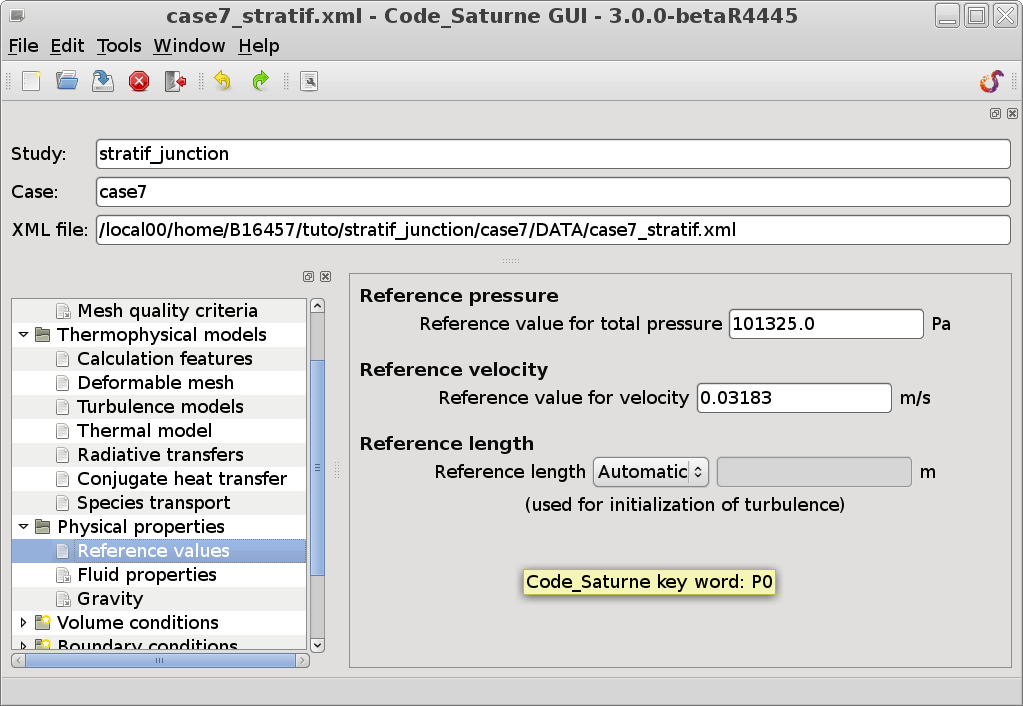
\includegraphics[width=12cm]{case5-V1}
\caption{Thermophysical models - Initialization}
\label{fig1_e5}
\end{center}
\end{figure}


\newpage
In the item {\itshape Fluid properties}, under the heading {\itshape Physical
properties}, enter the following information:

\begin{center}
\begin{tabular}{|c|c|c|}
\hline
Variable & Type & Value \\
\hline
\hline
Density & user law & $998.671\ kg.m^{-3} $ \\
\hline
Viscosity & user law & $0.445\times 10^{-4}\ kg.m^{-1}.s^{-1} $ \\
\hline
Specific Heat & Constant & $4\,182.88\ J.kg^{-1}.\mbox{\degresC}^{-1} $ \\
\hline
Thermal Conductivity & Constant & $0.601498\ W.m^{-1}.K^{-1}$\\
\hline
\end{tabular}
\end{center}

For density and viscosity, the value given here will serve as a reference
value (see user manual for details).

\begin{figure}[h!]
\begin{center}
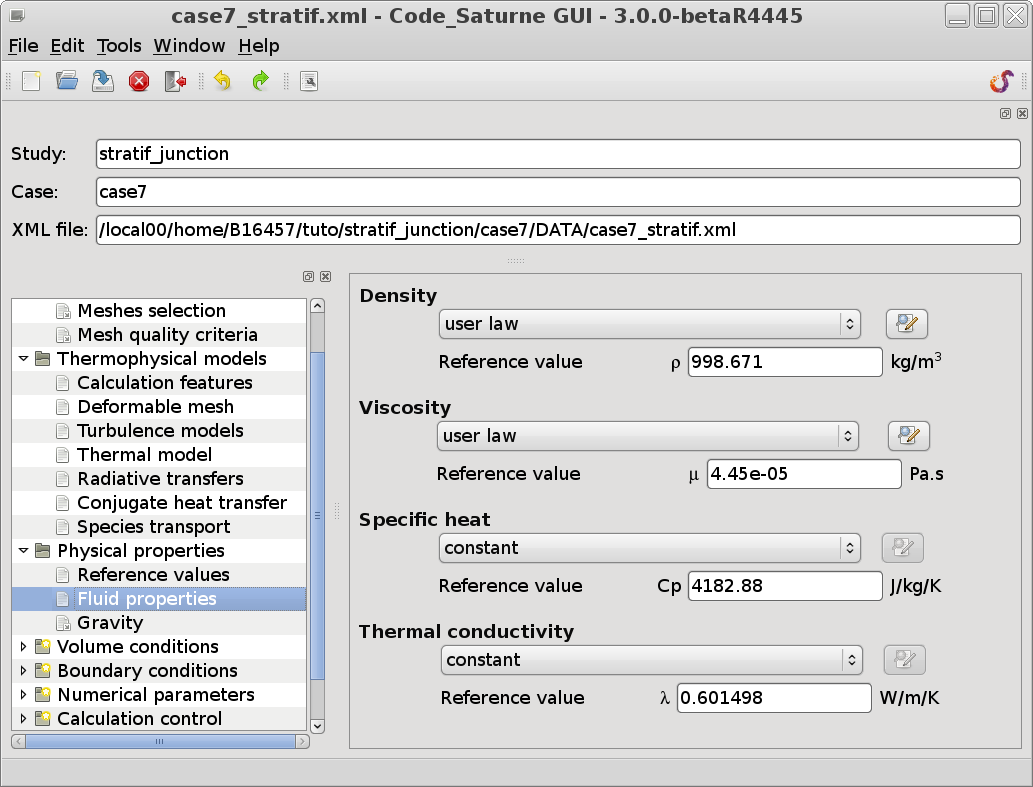
\includegraphics[width=12cm]{case5-V2}
\caption{Physical properties: fluid properties}
\label{fig2_e5}
\end{center}
\end{figure}

\newpage
For the density and viscosity, enter the expressions of the user laws as showed in
figures \ref{fig5_var1} and \ref{fig5_var2}, in the windows poping while clicking on the highlighted boxes.

\begin{figure}[h!]
\begin{center}
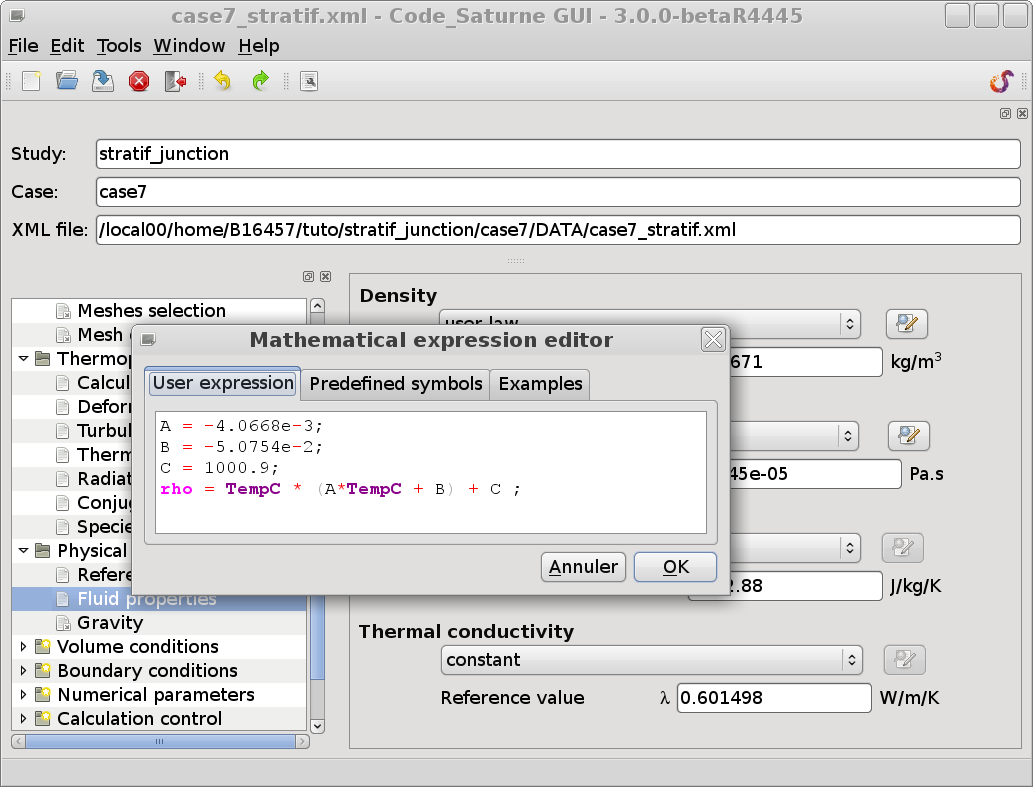
\includegraphics[width=12cm]{case5-V3}
\caption{Variable density}
\label{fig5_var1}
\end{center}
\end{figure}

\begin{figure}[h!]
\begin{center}
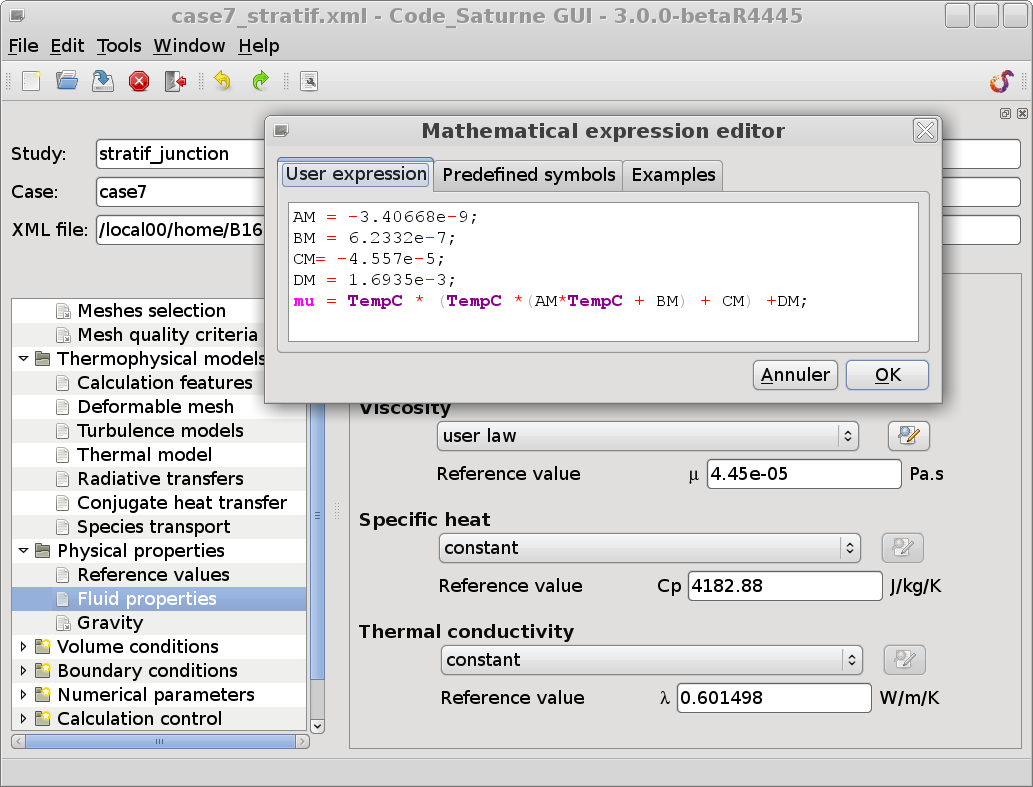
\includegraphics[width=12cm]{case5-V4}
\caption{Variable viscosity}
\label{fig5_var2}
\end{center}
\end{figure}

\newpage
The aim of the calculation is to simulate a stratified flow. It is therefore
necessary to have gravity. Set it to the right value in the item
{\itshape Gravity, hydrostatic pressure}.  In order to have a sharper
stratification, the pressure interpolation method will be set to
{\itshape improved}.

\begin{figure}[h!]
\begin{center}
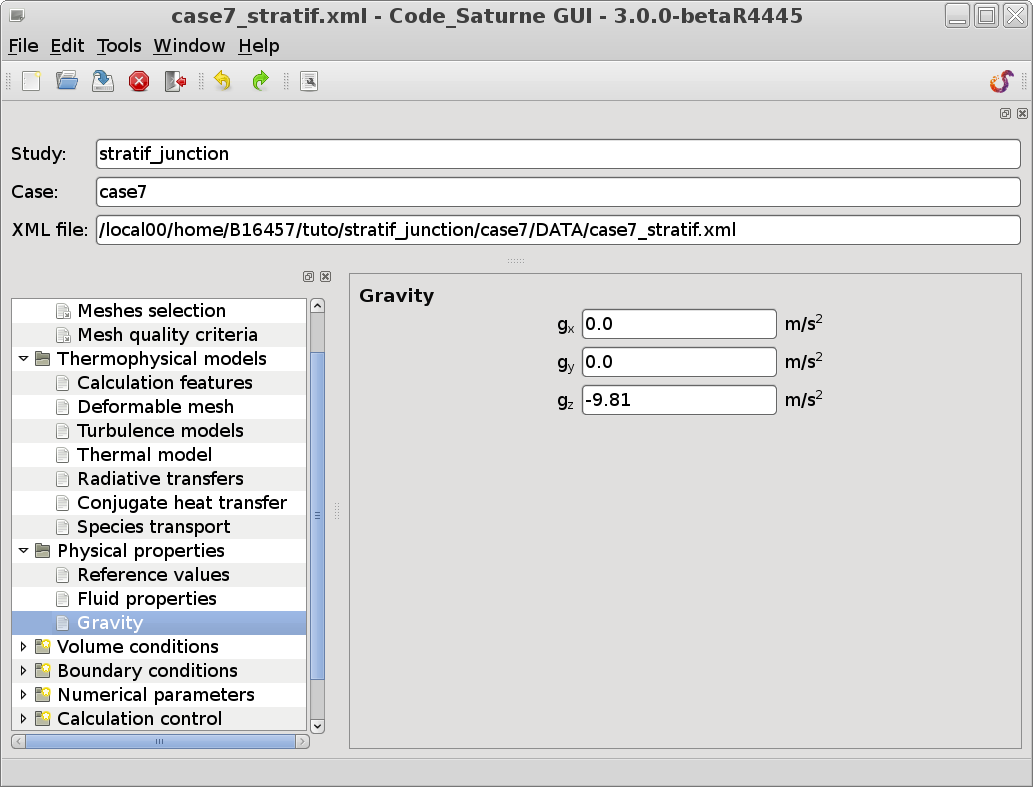
\includegraphics[width=12cm]{case5-V5}
\caption{Fluid properties - Gravity}
\label{fig3_e5}
\end{center}
\end{figure}


\newpage

Go to the item {\itshape Definition and initialization} under the heading
{\itshape Additional scalars} to specify the minimal and maximal values for the
temperature: 18.26\degresC\ and 38.5\degresC. Note that the initial value of
38.5\degresC\ set earlier is properly taken into account.

\begin{figure}[h!]
\begin{center}
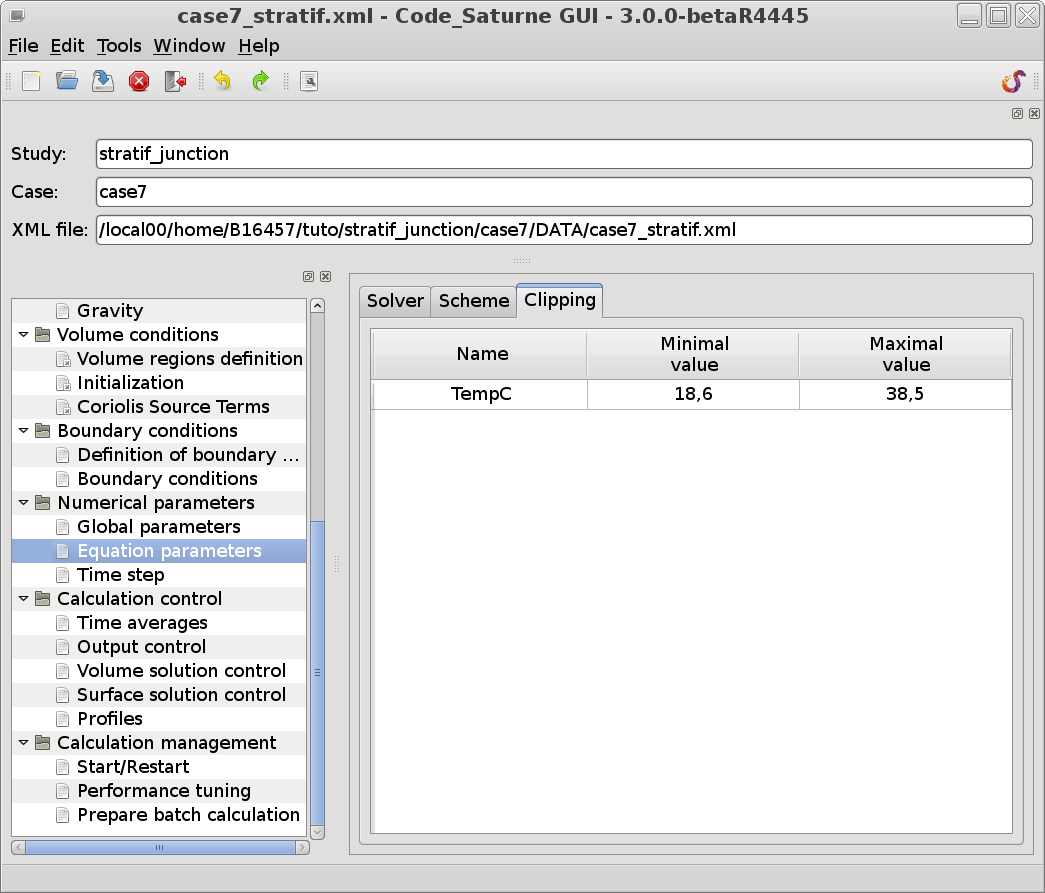
\includegraphics[width=12cm]{case5-V5b}
\caption{Scalar initialization}
\label{fig4_e5}
\end{center}
\end{figure}


\newpage
Create the boundary regions.

\begin{center}
\begin{tabular}{|c|c|}
\hline
Colors & Conditions \\
\hline
2 & inlet \\
\hline
6 & inlet \\
\hline
7 & outlet \\
\hline
5 & wall \\
\hline
\end{tabular}
\end{center}

\begin{figure}[h!]
\begin{center}
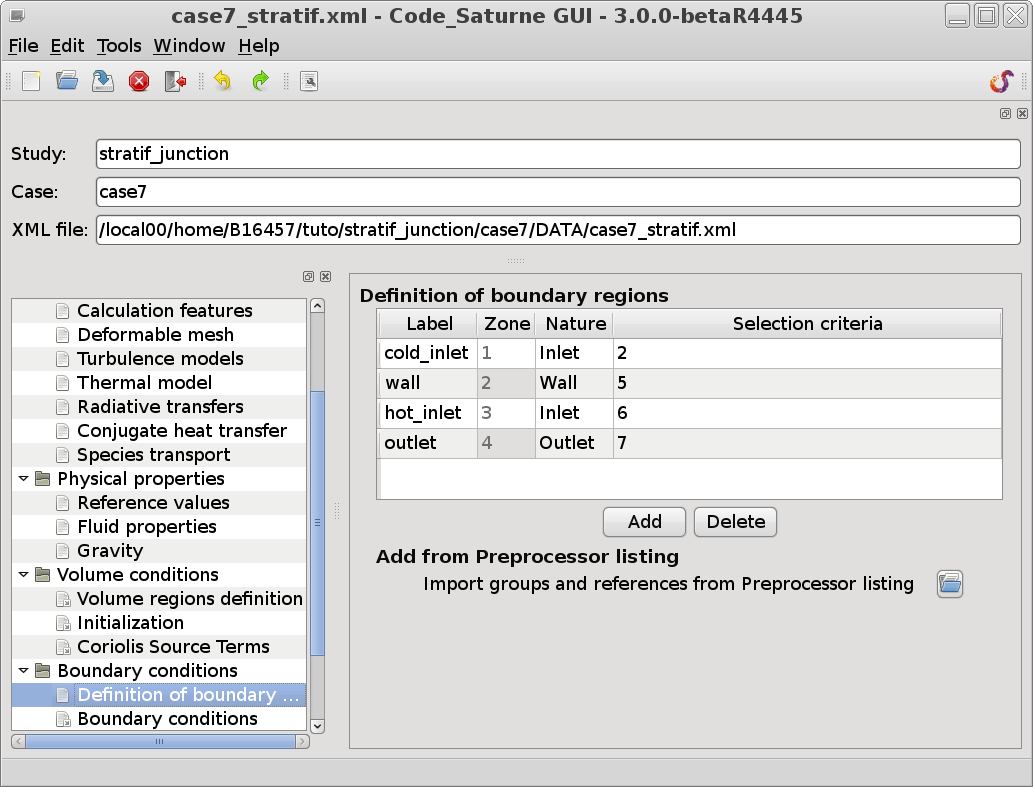
\includegraphics[width=12cm]{case5-V6}
\caption{Boundary regions}
\label{fig5_e5}
\end{center}
\end{figure}


\newpage
For the dynamic boundary conditions, the velocity is $0.03183\ m.s^{-1}$ in the
$z$ direction and the hydraulic diameter $0.4\ m$ for both inlets.


\begin{figure}[h!]
\begin{center}
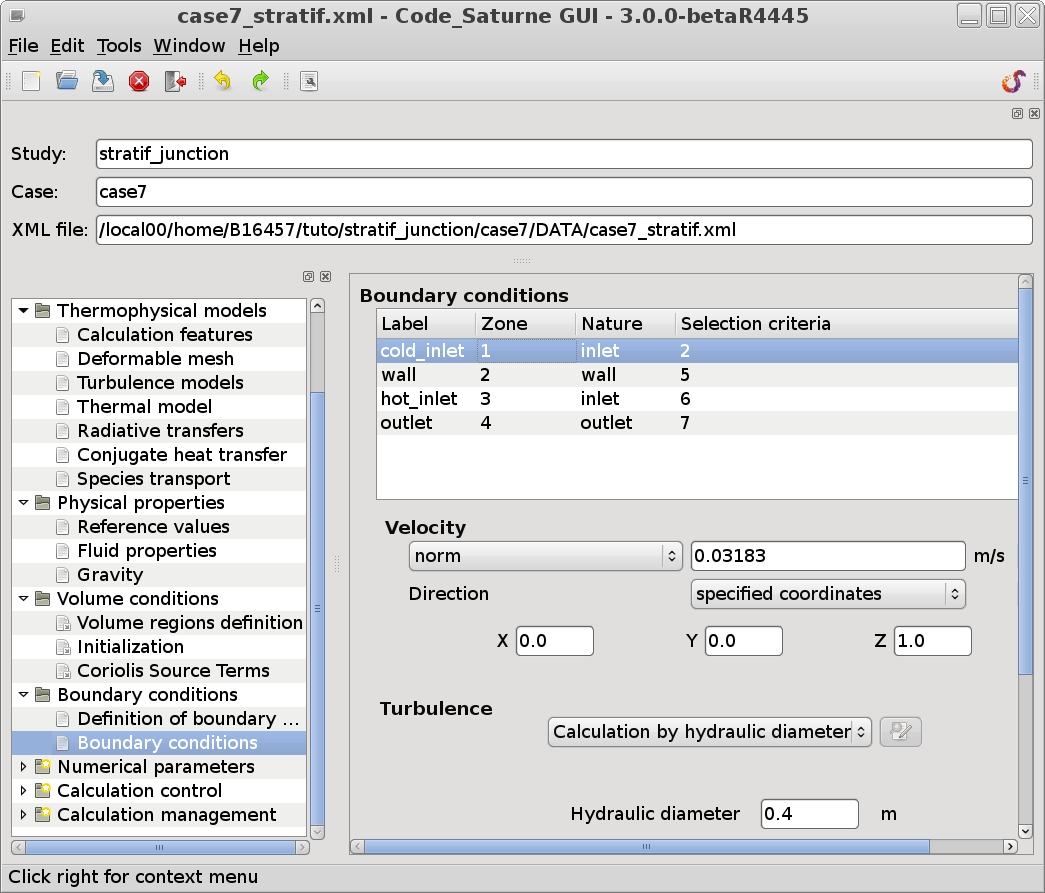
\includegraphics[width=10cm]{case5-V7}
\caption{Dynamic boundary conditions}
\label{fig6_e5}
\end{center}
\end{figure}

\begin{figure}[h!]
\begin{center}
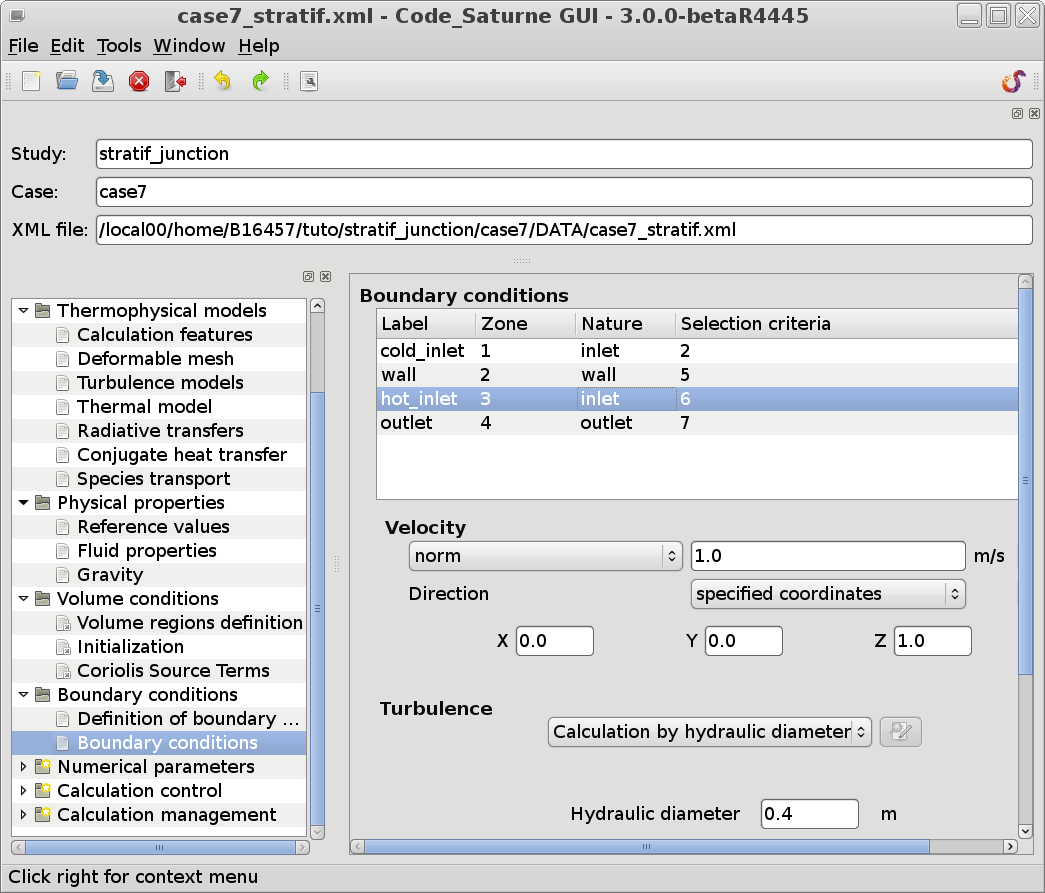
\includegraphics[width=10cm]{case5-V8}
\caption{Dynamic boundary conditions}
\label{fig6_e5}
\end{center}
\end{figure}

\newpage
For the scalar boundary conditions, the temperature of the cold inlet is
18.6\degresC\ and that of the hot inlet is 38.5\degresC.\\
\fbox{\begin{minipage}{\textwidth}\texttt{
- {\bf Cold inlet:}
}\end{minipage} }

\begin{figure}[h!]
\begin{center}
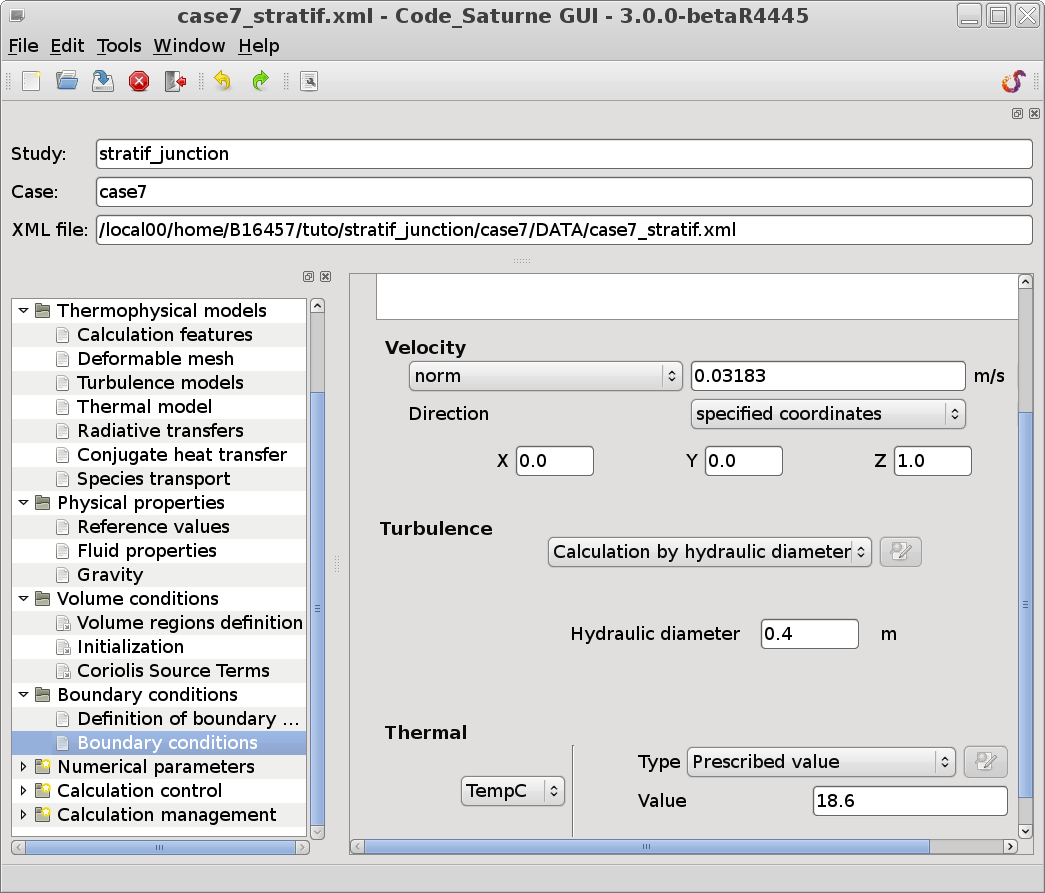
\includegraphics[width=10cm]{case5-V9}
\caption{Temperature boundary conditions}
\label{fig8_e5}
\end{center}
\end{figure}

\fbox{\begin{minipage}{\textwidth}\texttt{
- {\bf Hot inlet:}
}\end{minipage} }

\begin{figure}[h!]
\begin{center}
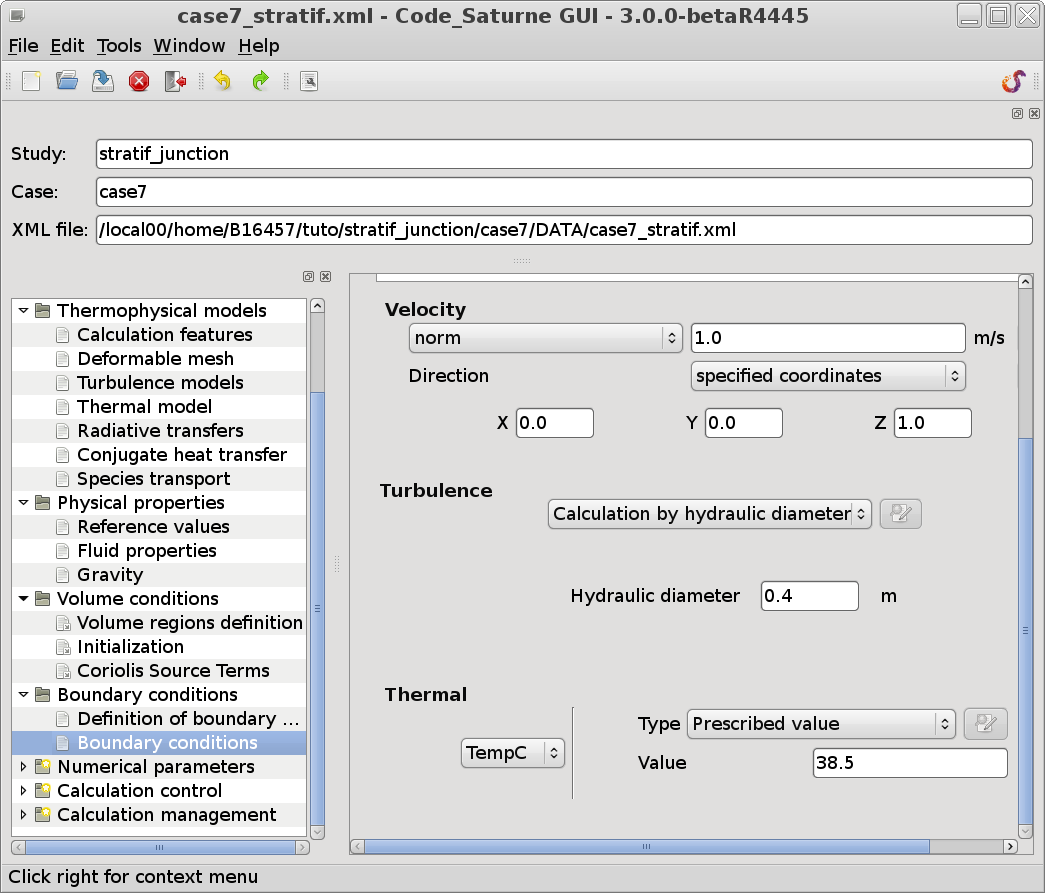
\includegraphics[width=10cm]{case5-V10}
\caption{Temperature boundary conditions}
\label{fig8_e5}
\end{center}
\end{figure}

\newpage
Tick the appropriate box for the time step to be variable in time and uniform in
space. In the boxes below, enter the following parameters:
\begin{center}
\begin{tabular}{|l|c|}
\hline
\multicolumn{2}{|c|}{Parameters of calculation control} \\
\hline
Number of iterations & 100 \\
\hline
Reference time step & $1\ s$ \\
\hline
Maximal CFL number & 20 \\
\hline
Maximal Fourier number & 60 \\
\hline
Minimal time step & $0.01\ s$ \\
\hline
Maximal time step & $70\ s$ \\
\hline
Time step maximal variation & $0.1$ \\
\hline
\end{tabular}\\
\end{center}

And activate the option
{\itshape Time step limitation with the local thermal time step}

\begin{figure}[h!]
\begin{center}
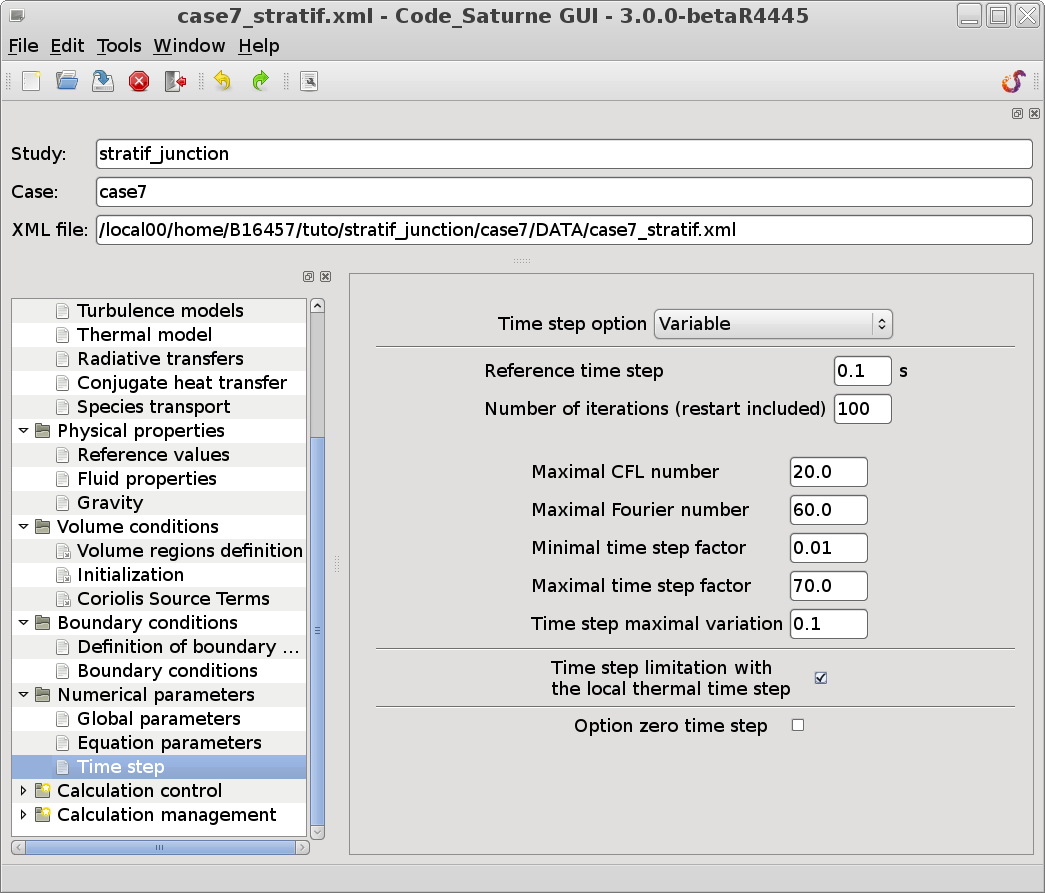
\includegraphics[width=13cm]{case5-V11}
\caption{Time step}
\label{fig11_e5}
\end{center}
\end{figure}


\newpage
Set the frequency of post-processing for the main writer {\textbf results} to 10.

Create four monitoring probes at the following coordinates:
\begin{center}
\begin{tabular}{|c|c|c|c|}
\hline
Points & X(m) & Y(m) & Z(m)\\
\hline
1 & 0.010025 & 0.01534 & -0.011765 \\
\hline
2 & 1.625 & 0.01534 & -0.031652 \\
\hline
3 & 3.225 & 0.01534 & -0.031652 \\
\hline
4 & 3.8726 & 0.047481 & 7.25 \\
\hline
\end{tabular}
\end{center}

\begin{figure}[h!]
\begin{center}
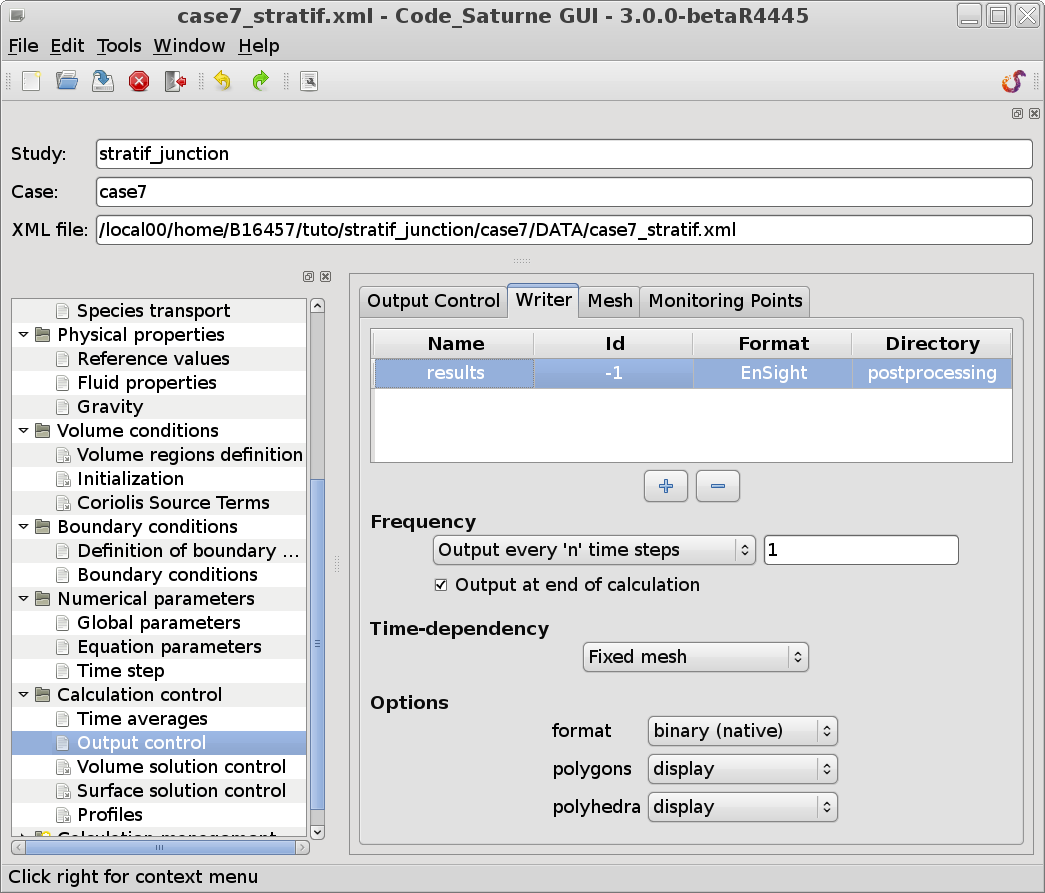
\includegraphics[width=12cm]{case5-V12}
\caption{Output management}
\label{fig12_e5}
\end{center}
\end{figure}

\begin{figure}[h!]
\begin{center}
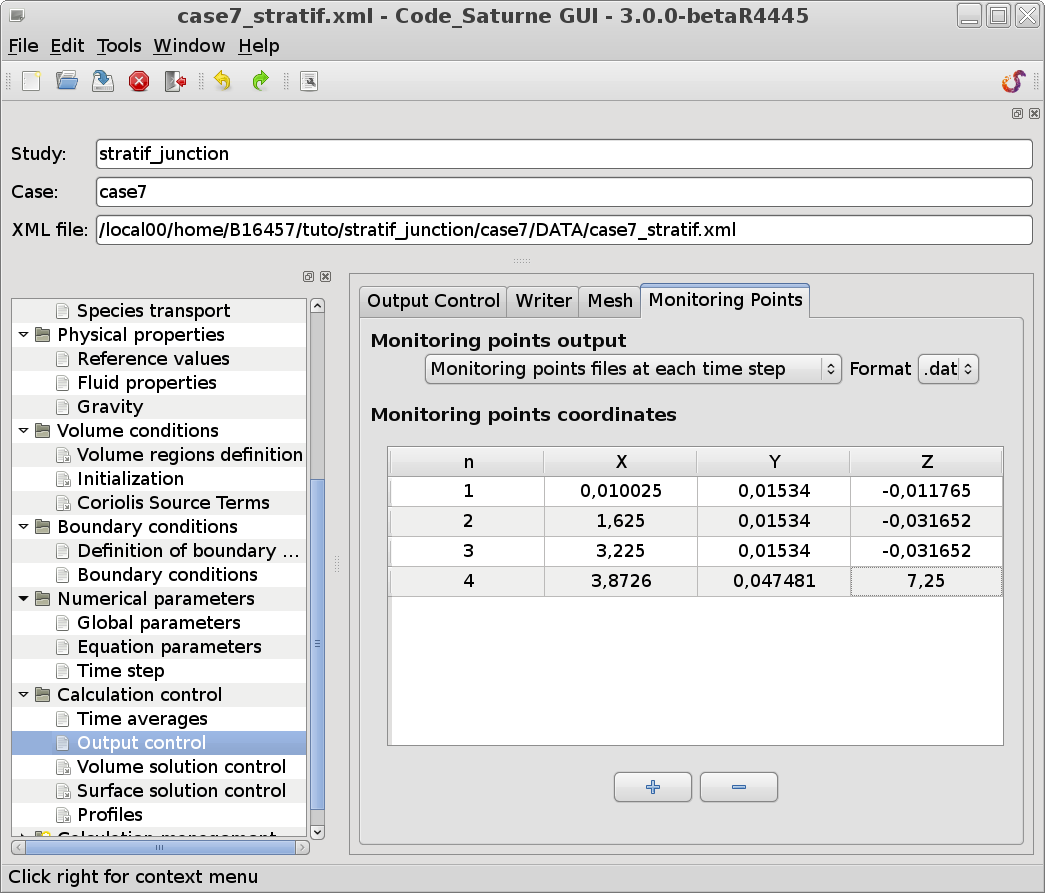
\includegraphics[width=12cm]{case5-V13}
\caption{Monitoring points}
\label{fig12bis_e5}
\end{center}
\end{figure}

\newpage
For the advanced post-processing features, copy the files
{\itshape cs\_user\_postprocess.c} and {\itshape cs\_user\_postprocess\_var.f90} to the SRC
directory. The general content of these routines is described in the user manual
or in the examples available in the directory \texttt{SRC/REFERENCE/base}. The modified
routines adapted to this test case are available in the \texttt{examples}
directory. Only the main elements are mentioned here.

$\bullet$ {\bfseries cs\_user\_postprocess\_meshes} (in  {\bfseries cs\_user\_postprocess.c})\\
This  is called only once, at the beginning of the calculation. It allows
to define the different writers and parts.

$\bullet$ {\bfseries cs\_user\_postprocess\_var.f90}\\
This routine is called at each time step. It allows to specify which variable
will be written on which part.

